\documentclass[style=sailor,size=12pt]{powerdot}
\usepackage{epic,array,ecltree,url,calrsfs}
\usepackage[nointegrals]{wasysym}
\usepackage{listings}
\usepackage{epsfig}
\usepackage{amsmath}
\usepackage{amsfonts}
\usepackage{amssymb}
\usepackage{amsxtra}
\usepackage{amsthm}
\usepackage{mlextra} % Must be below ams packages
\usepackage{mathrsfs}
\usepackage{color}
\usepackage{array}
\usepackage{graphicx}
\graphicspath{ {../art/} }
\usepackage{bm}
\usepackage{tikz}
\usepackage{multicol}
\usepackage{enumitem}
\usepackage{blkarray}
\usepackage{bigstrut}
\setlength{\bigstrutjot}{4pt}
\usetikzlibrary{arrows}
\usepackage{subcaption}

\pdsetup{method=normal}

\title{Review: Relations and Functions}
\author{Foundations of Computer Science}
\date{\today}

\begin{document}
\maketitle
\section[slide=true]{Relations}
\begin{slide}[bm=,toc=]{Definition}
\begin{defn}{A.19}[Ben Ari]
An \emph{n-ary relation} $\mathcal{R}$ is a subset of $S_1 \times \cdots \times
S_n$. 
\begin{itemize}
\item $\mathcal{R}$ is said to be a relation \emph{on} $S_1 \times \cdots \times
S_n$.
\item The value of $n$ is called the ``arity'' of the relation.
\item If all the sets $S_i$ are the same set $S$, $\mathcal{R}$ is said to be
an \emph{n-ary} relation on $S$.
\begin{itemize}
\item In this case $\mathcal{R}$ is called a \emph{homogenous} relation.
\end{itemize}
\item A 1-ary (unary) relation is simply a subset.
\end{itemize}
\end{defn}
\end{slide}

\begin{slide}[bm=,toc=]{Examples of Binary Relations}
\begin{ex}{}[Explicit]~\\
\begin{itemize}
\item Let $L = \{a,b,c\}$.
\item Let $W = \{all,ball,bat,cat\}$.
\item The we can define binary relation $R \subseteq L \times W$ such that 
      $R = \{(a,all),(b,ball),(b, bat), (c,cat)\}$.
\end{itemize}
\end{ex}
\begin{ex}{}[Set Comprehension]~\\
\begin{itemize}
\item Let $\Sigma = \{a,b\}$.
\item Let $S = \Sigma^0 \cup \Sigma \cup \Sigma^2$
\item Define binary relation $R_{pre}$ on $S$ such that:
      $R_{pre} = \{(x,y)| y = xw \text{ for some } w \in S \}$.
\end{itemize}
\end{ex}

\end{slide}

\begin{slide}[bm=,toc=]{Matrix Representations of Relations}
Relations can be represented using a binary matrix in which the
value corresponding to a tuple is set to $1$ if the tuple is
in the relation, and $0$ otherwise.
\begin{ex}{}[$R$ and $R_{pre}$ from previous slide]
\[
R = 
\begin{blockarray}{cccc}
\begin{block}{cccc}
& a & b & c \\
\end{block}
\begin{block}{c[ccc]}
all  & 1 & 0 & 0 \bigstrut[t] \\
ball & 0 & 1 & 0 \\
bat  & 0 & 1 & 0 \\
cat  & 0 & 0 & 1 \\
\end{block}
\end{blockarray}
\qquad R_{pre} =
\begin{blockarray}{cccccccc}
\begin{block}{cccccccc}
 & \epsilon & a & b & aa & ab & ba & bb \\
\end{block}
\begin{block}{c[ccccccc]}
\epsilon & 1  & 1 & 1 & 1  & 1  & 1  & 1\bigstrut[t] \\
a  & 0& 1 & 0 & 1  & 1  & 0  & 0 \\
b  & 0& 0 & 1 & 0  & 0  & 1  & 1 \\
aa & 0& 0 & 0 & 1  & 0  & 0  & 0 \\
ab & 0& 0 & 0 & 0  & 1  & 0  & 0 \\
ba & 0& 0 & 0 & 0  & 0  & 1  & 0 \\
bb & 0& 0 & 0 & 0  & 0  & 0  & 1 \\
\end{block}
\end{blockarray}
\]
\end{ex}
\end{slide}

\begin{slide}[bm=,toc=]{DiGraph Representations of Relations}
Binary relations can also be represented using a directed graph in which
vertices represent elements and edges are placed between vertices
if their corresponding tuple is in the relation.
\begin{ex}{}[$R$ and $R_{pre}$ from previous slide]
~\\
\vspace{-2mm}
\begin{figure}[h!]
\centering
\subcaptionbox*{$R$}[.3\linewidth]{
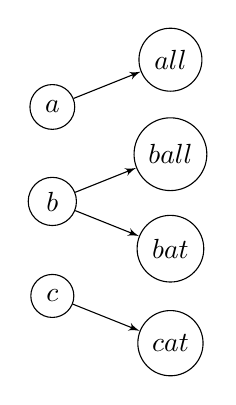
\begin{tikzpicture}
\tikzset{vertex/.style = {shape=circle,draw,minimum size=1.5em}}
\tikzset{edge/.style = {->,> = latex'}}

\node[vertex](c1) at (0,0.6) {$c$};
\node[vertex](b1) at (0,1.8) {$b$};
\node[vertex](a1) at (0,3) {$a$};
\node[vertex](d2) at (1.5,0) {$cat$};
\node[vertex](c2) at (1.5,1.2) {$bat$};
\node[vertex](b2) at (1.5,2.4) {$ball$};
\node[vertex](a2) at (1.5,3.6) {$all$};

\draw[edge] (a1) to (a2);
\draw[edge] (b1) to (b2);
\draw[edge] (b1) to (c2);
\draw[edge] (c1) to (d2);
\end{tikzpicture}
}
\subcaptionbox*{$R_{pre}$}[.5\linewidth]{
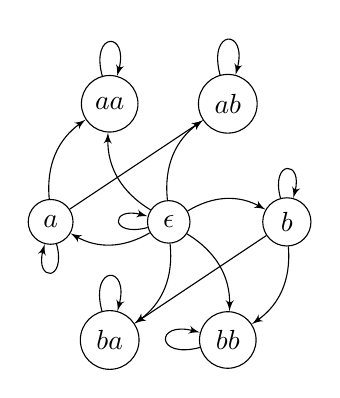
\begin{tikzpicture}
\tikzset{vertex/.style = {shape=circle,draw,minimum size=1.5em}}
\tikzset{edge/.style = {->,> = latex'}}

\node[vertex](aa) at (0.75,3) {$aa$};
\node[vertex](ab) at (2.25,3) {$ab$};
\node[vertex](a) at (0,1.5) {$a$};
\node[vertex](e) at (1.5,1.5) {$\epsilon$};
\node[vertex](b) at (3,1.5) {$b$};
\node[vertex](ba) at (0.75,0) {$ba$};
\node[vertex](bb) at (2.25,0) {$bb$};

\draw[edge] (a) to[loop below] (a);
\draw[edge] (b) to[loop above] (b);
\draw[edge] (e) to[loop left] (e);
\draw[edge] (aa) to[loop above] (aa);
\draw[edge] (ab) to[loop above] (ab);
\draw[edge] (ba) to[loop above] (ba);
\draw[edge] (bb) to[loop left] (bb);
\draw[edge] (e) to[bend left] (a);
\draw[edge] (e) to[bend left] (b);
\draw[edge] (e) to[bend left] (aa);
\draw[edge] (e) to[bend left] (ab);
\draw[edge] (e) to[bend left] (ba);
\draw[edge] (e) to[bend left] (bb);
\draw[edge] (a) to[bend left] (aa);
\draw[edge] (a) to (ab);
\draw[edge] (b) to (ba);
\draw[edge] (b) to[bend left] (bb);
\end{tikzpicture}
}
\end{figure}

\end{ex}
\end{slide}


\begin{slide}[bm=,toc=]{Reflexive Relations}
\begin{defn}{A.21}[Ben Ari]
Let $R$ be a binary relation on $S$.
\\~\\
$R$ is \emph{reflexive} if and only if $R(x,x)$ for all $x \in S$.
\end{defn}
~
\vspace{-12mm}
\pause \begin{figure}[t]
\caption*{\textbf{Example:} $R_{pre}$ is a reflexive relation on $S = \{\epsilon,a,b,aa,bb\}$} 
\pause \subcaptionbox*{As Matrix}{
$ \begin{blockarray}{cccccc}
 \begin{block}{cccccc}
  & \epsilon & a & b & aa & bb \\
 \end{block}
 \begin{block}{c[ccccc]}
 \epsilon & 1 & 1 & 1 & 1 & 1 \bigstrut[t] \\
 a        & 0 & 1 & 0 & 1 & 0  \\
 b        & 0 & 0 & 1 & 0 & 1  \\
 aa       & 0 & 0 & 0 & 1 & 0  \\
 bb       & 0 & 0 & 0 & 0 & 1  \\
 \end{block}
 \end{blockarray} $
}
\qquad
\pause \subcaptionbox*{As Digraph}{
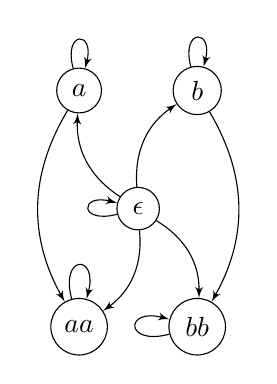
\begin{tikzpicture}
\tikzset{vertex/.style = {shape=circle,draw,minimum size=1.5em}}
\tikzset{edge/.style = {->,> = latex'}}

\node[vertex](a) at (0.75,3) {$a$};
\node[vertex](b) at (2.25,3) {$b$};
\node[vertex](e) at (1.5,1.5) {$\epsilon$};
\node[vertex](aa) at (0.75,0) {$aa$};
\node[vertex](bb) at (2.25,0) {$bb$};

\draw[edge] (a) to[loop above] (a);
\draw[edge] (b) to[loop above] (b);
\draw[edge] (e) to[loop left] (e);
\draw[edge] (aa) to[loop above] (aa);
\draw[edge] (bb) to[loop left] (bb);
\draw[edge] (e) to[bend left] (a);
\draw[edge] (e) to[bend left] (b);
\draw[edge] (e) to[bend left] (aa);
\draw[edge] (e) to[bend left] (bb);
\draw[edge] (a) to[bend right] (aa);
\draw[edge] (b) to[bend left] (bb);
\end{tikzpicture}
}
\end{figure}

\end{slide}

\begin{slide}[bm=,toc=]{Symmetric Relations}
\begin{defn}{A.21}[Ben Ari]
Let $R$ be a binary relation on $S$.
\\~\\
$R$ is \emph{symmetric} if and only if $R(x_1,x_2)$ implies $R(x_2,x_1)$.
\end{defn}
~
\vspace{-12mm}
\pause \begin{figure}[t]
\caption*{\textbf{Example:} $R_l$ is a symmetric relation on $S = \{\epsilon,a,b,aa,bb\}$} 
\pause \subcaptionbox*{As Matrix}{
$ \begin{blockarray}{cccccc}
 \begin{block}{cccccc}
  & \epsilon & a & b & aa & bb \\
 \end{block}
 \begin{block}{c[ccccc]}
 \epsilon & 1 & 0 & 0 & 0 & 0 \bigstrut[t] \\
 a        & 0 & 1 & 1 & 0 & 0  \\
 b        & 0 & 1 & 1 & 0 & 0  \\
 aa       & 0 & 0 & 0 & 1 & 1  \\
 bb       & 0 & 0 & 0 & 1 & 1  \\
 \end{block}
 \end{blockarray} $
}
\qquad
\pause \subcaptionbox*{As Digraph}{
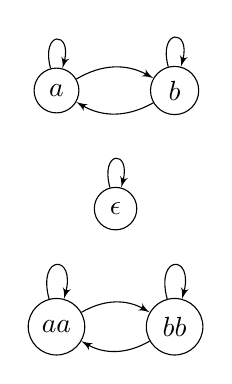
\begin{tikzpicture}
\tikzset{vertex/.style = {shape=circle,draw,minimum size=1.5em}}
\tikzset{edge/.style = {->,> = latex'}}

\node[vertex](a) at (0.75,3) {$a$};
\node[vertex](b) at (2.25,3) {$b$};
\node[vertex](e) at (1.5,1.5) {$\epsilon$};
\node[vertex](aa) at (0.75,0) {$aa$};
\node[vertex](bb) at (2.25,0) {$bb$};

\draw[edge] (a) to[loop above] (a);
\draw[edge] (b) to[loop above] (b);
\draw[edge] (e) to[loop above] (e);
\draw[edge] (aa) to[loop above] (aa);
\draw[edge] (bb) to[loop above] (bb);
\draw[edge] (a) to[bend left] (b);
\draw[edge] (b) to[bend left] (a);
\draw[edge] (bb) to[bend left] (aa);
\draw[edge] (aa) to[bend left] (bb);
\end{tikzpicture}
}
\end{figure}
\pause {\footnotesize Exercise: Give a rule for the relation.} 
\pause {\footnotesize \textbf{Ans:} $R_{l} = \{(x,y)| |x| = |y|\}$}
\end{slide}

\begin{slide}[bm=,toc=]{Antisymmetric Relations}
\begin{defn}{A.21}[Ben Ari]
Let $R$ be a binary relation on $S$.
\\~\\
$R$ is \emph{antisymmetric} if and only if $(x_1,x_2) \in R$ and $(x_2,x_1) \in
R$ implies $x_1 = x_2$.
\end{defn}
~
\vspace{-12mm}
\pause \begin{figure}[t]
\caption*{\textbf{Example:} $R_{pre}$ is also antisymmetric on $S = \{\epsilon,a,b,aa,bb\}$} 
\subcaptionbox*{As Matrix}{
$ \begin{blockarray}{cccccc}
 \begin{block}{cccccc}
  & \epsilon & a & b & aa & bb \\
 \end{block}
 \begin{block}{c[ccccc]}
 \epsilon & 1 & 1 & 1 & 1 & 1 \bigstrut[t] \\
 a        & 0 & 1 & 0 & 1 & 0  \\
 b        & 0 & 0 & 1 & 0 & 1  \\
 aa       & 0 & 0 & 0 & 1 & 0  \\
 bb       & 0 & 0 & 0 & 0 & 1  \\
 \end{block}
 \end{blockarray} $
}
\qquad
\subcaptionbox*{As Digraph}{
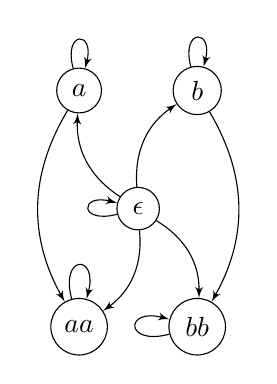
\begin{tikzpicture}
\tikzset{vertex/.style = {shape=circle,draw,minimum size=1.5em}}
\tikzset{edge/.style = {->,> = latex'}}

\node[vertex](a) at (0.75,3) {$a$};
\node[vertex](b) at (2.25,3) {$b$};
\node[vertex](e) at (1.5,1.5) {$\epsilon$};
\node[vertex](aa) at (0.75,0) {$aa$};
\node[vertex](bb) at (2.25,0) {$bb$};

\draw[edge] (a) to[loop above] (a);
\draw[edge] (b) to[loop above] (b);
\draw[edge] (e) to[loop left] (e);
\draw[edge] (aa) to[loop above] (aa);
\draw[edge] (bb) to[loop left] (bb);
\draw[edge] (e) to[bend left] (a);
\draw[edge] (e) to[bend left] (b);
\draw[edge] (e) to[bend left] (aa);
\draw[edge] (e) to[bend left] (bb);
\draw[edge] (a) to[bend right] (aa);
\draw[edge] (b) to[bend left] (bb);
\end{tikzpicture}
}
\end{figure}
\end{slide}

\begin{slide}[bm=,toc=]{Transitive Relations}
\begin{defn}{A.21}[Ben Ari]
Let $R$ be a binary relation on $S$.
\\~\\
$R$ is \emph{transitive} if and only if $R(x_1,x_2)$ and $R(x_2,x_3)$ implies $R(x_1,x_3)$.
\end{defn}
~
\vspace{-12mm}
\pause \begin{figure}[t]
\caption*{\textbf{Example:} Both $R_{pre}$ and $R_l$ are transitive on $S = \{\epsilon,a,b,aa,bb\}$} 
\subcaptionbox*{$R_{pre}$}{
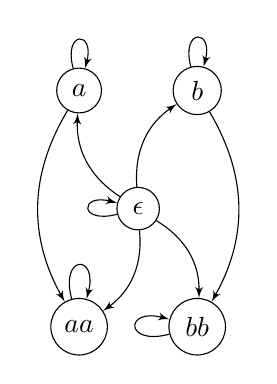
\begin{tikzpicture}
\tikzset{vertex/.style = {shape=circle,draw,minimum size=1.5em}}
\tikzset{edge/.style = {->,> = latex'}}

\node[vertex](a) at (0.75,3) {$a$};
\node[vertex](b) at (2.25,3) {$b$};
\node[vertex](e) at (1.5,1.5) {$\epsilon$};
\node[vertex](aa) at (0.75,0) {$aa$};
\node[vertex](bb) at (2.25,0) {$bb$};

\draw[edge] (a) to[loop above] (a);
\draw[edge] (b) to[loop above] (b);
\draw[edge] (e) to[loop left] (e);
\draw[edge] (aa) to[loop above] (aa);
\draw[edge] (bb) to[loop left] (bb);
\draw[edge] (e) to[bend left] (a);
\draw[edge] (e) to[bend left] (b);
\draw[edge] (e) to[bend left] (aa);
\draw[edge] (e) to[bend left] (bb);
\draw[edge] (a) to[bend right] (aa);
\draw[edge] (b) to[bend left] (bb);
\end{tikzpicture}
}
\qquad
\subcaptionbox*{$R_l$}{
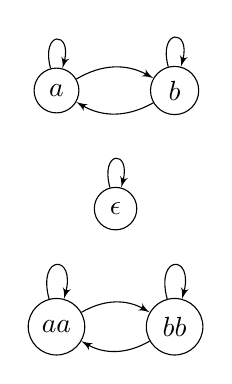
\begin{tikzpicture}
\tikzset{vertex/.style = {shape=circle,draw,minimum size=1.5em}}
\tikzset{edge/.style = {->,> = latex'}}

\node[vertex](a) at (0.75,3) {$a$};
\node[vertex](b) at (2.25,3) {$b$};
\node[vertex](e) at (1.5,1.5) {$\epsilon$};
\node[vertex](aa) at (0.75,0) {$aa$};
\node[vertex](bb) at (2.25,0) {$bb$};

\draw[edge] (a) to[loop above] (a);
\draw[edge] (b) to[loop above] (b);
\draw[edge] (e) to[loop above] (e);
\draw[edge] (aa) to[loop above] (aa);
\draw[edge] (bb) to[loop above] (bb);
\draw[edge] (a) to[bend left] (b);
\draw[edge] (b) to[bend left] (a);
\draw[edge] (bb) to[bend left] (aa);
\draw[edge] (aa) to[bend left] (bb);
\end{tikzpicture}
}
\end{figure}
\end{slide}
\begin{slide}[bm=,toc=]{Equivalence Relations}
\begin{defn}{--- Equivalence Relations}~\\
A relation is an equivalence relation if it is:

\begin{itemize}
\item Reflexive
\item Symmetric
\item Transitive
\end{itemize}
\end{defn}
\textbf{Examples}:
\begin{itemize}
\item $\{(x,y) | x = y \}$
\item $\{(x,y) | x \text{ and } y \text{ begin with the same character}\}$
\item $\{(x,y) | x \text{ and } y \text{ contain the same substring}\}$
\item $R_{l}$ 
\end{itemize}
\end{slide}

\begin{slide}[bm=,toc=]{Partial Orders}
\begin{defn}{--- Partial Orders}~\\
A relation is a partial order if it is:

\begin{itemize}
\item Reflexive
\item Antisymmetric
\item Transitive
\end{itemize}
\textbf{Examples}:
\begin{itemize}
\item $R_{pre}$
\item $\{(x,y) | x \text{ is a substring of } y \}$
\item $\{(x,y) | x \text{ is a subset of } y \}$
\item $\{(x,y) | y \text{ is a suffix of } x \}$
\end{itemize}
\end{defn}
\end{slide}
\begin{slide}[bm=,toc=]{Combining Relations}
\begin{itemize}
\item Relations are sets.
\item Therefore, they can be combined using set operations.
\item That is, given arbitrary relations $R_1$ and $R_2$, we can form:
\begin{itemize}
\item $R_1 \cup R_2$
\item $R_1 \cap R_2$
\item $R_1 - R_2$
\item $R_2 - R_1$
\end{itemize}
\item Note that $R_1$ and $R_2$ must have the same arity.
\end{itemize}
\end{slide}

\begin{slide}[bm=,toc=]{Composition of Binary Relations}
We can also combine binary relations using the \emph{composition} operation, denoted
$R_1 \circ R_2$.
\begin{itemize}
\item Assume $R_2$ is a relation on $S_1 \times S_2$ and $R_1$ is a relation on
$S_3 \times S_4$.
\item Let $S = S_2 \cap S_3$.
\item The composition forms a new relation on $S_1 \times S_4$, such that:
\begin{itemize}
\item $(x,z) \in R_1 \circ R_2$ if and only if there exists $y$ in $S$ such
that $(y,z) \in R_1$ and $(x,y) \in R_2$.
\end{itemize}
\item Note that in the case where $S = \emptyset$, $R_1 \circ R_2$ is also empty.
\end{itemize}
\vspace{-5mm}
\begin{figure}[b]
\begin{subfigure}{.4\linewidth}
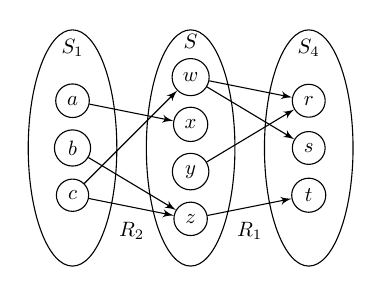
\begin{tikzpicture}[scale=.75, every node/.style={scale=.75}]
\tikzset{vertex/.style = {shape=circle,draw,minimum size=1.5em}}
\tikzset{edge/.style = {->,> = latex'}}

\draw (0, 1.2) ellipse (.75cm and 2cm);
\node[vertex](c) at (0,0.4) {$c$};
\node[vertex](b) at (0,1.2) {$b$};
\node[vertex](a) at (0,2) {$a$};
\node (s1) at (0, 2.9) {$S_1$};

\node (r2) at (1, -0.2) {$R_2$};

\draw (2, 1.2) ellipse (.75cm and 2cm);
\node[vertex](z) at (2,0) {$z$};
\node[vertex](y) at (2,0.8) {$y$};
\node[vertex](x) at (2,1.6) {$x$};
\node[vertex](w) at (2,2.4) {$w$};
\node (s) at (2, 3) {$S$};

\node (r1) at (3, -0.2) {$R_1$};

\draw (4, 1.2) ellipse (.75cm and 2cm);
\node[vertex](t) at (4,0.4) {$t$};
\node[vertex](s) at (4,1.2) {$s$};
\node[vertex](r) at (4,2) {$r$};
\node (s4) at (4, 2.9) {$S_4$};



\draw[edge] (a) to (x);
\draw[edge] (b) to (z);
\draw[edge] (c) to (w);
\draw[edge] (c) to (z);

\draw[edge] (w) to (r);
\draw[edge] (w) to (s);
\draw[edge] (z) to (t);
\draw[edge] (y) to (r);

\end{tikzpicture}

\end{subfigure}
\begin{subfigure}{.5\linewidth}
\begin{align*}
  =& R_1 \circ R_2 \\
  =& \{(b,t),(c,r),(c,s),(c,t)\}
\end{align*}
\end{subfigure}
\end{figure}

\end{slide}
\begin{slide}[bm=,toc=]{Powers of Binary Relations}
\begin{defn}{-- Powers of Relations}
~\\
Let $R$ be a binary homogenous relation on $S$.
\\~\\
The relation $R^n$ is defined inductively by: 
\begin{itemize}
\item $R^1 = R$
\item $R^{n+1} = R^n \circ R$
\end{itemize}
\end{defn}
\textbf{Notes:}
\begin{itemize}
\item This definition makes use of the concept of relation composition
given on the previous slide.
\item Useful for defining paths of length $n$.
\item We will see it again in modal logic.
\end{itemize}
\end{slide}

\section[slide=true]{Functions}
\begin{slide}[bm=,toc=]{Definition}
\begin{defn}{A.23}[Ben Ari]
~\\
Let $\mathcal{F}$ be a relation on $S_1 \times \cdots \times S_n$.
\\~\\
$\mathcal{F}$ is a \emph{function} if and only if for every \emph{(n -- 1)-tuple}
$(x_1,...,x_{n-1}) \in S_1 \times \cdots \times S_{n-1}$, there is at most
one $x_n \in S_n$, such that $\mathcal{F}(x_1,...,x_n)$.
\begin{itemize}
\item For a function $\mathcal{F}$ we write $x_n = \mathcal{F}(x_1,...,x_{n-1})$.
\item The \emph{domain} of $\mathcal{F}$ is the set of all
$(x_1,...,x_{n-1})\in S_1 \times \cdots \times S_{n-1}$ for which (exactly one)
$x_n = \mathcal{F}(x_1,...,x_{n-1})$ exists.
\item The \emph{range} of $\mathcal{F}$ is the set of all $x_n \in S_n$ such
that $x_n = \mathcal{F}(x_1,...,x_{n-1})$ for at least one $(x_1,...,x_{n-1})$. 
\end{itemize}
\end{defn}
\end{slide}
\begin{slide}[bm=,toc=]{Examples of Functions}
\begin{itemize}
\item \textbf{As a Special Relation:}
\begin{itemize}
\item With explicit set notation: \[f_1 = \{(1,3),(2,1),(3,2)\}\]
\vspace{-5mm}
\item With set comprehension: \[f_2 = \{(n_1,n_2)|n_2 = n_1^2\}\]
\end{itemize}
\item \textbf{Functional Notation:}
\vspace{-3mm}
\[
  f_3(x) = x^2 + 1
  \]
\vspace{-5mm}
\item \textbf{Arrow Notation:}
\vspace{-3mm}
\begin{align*}
f_4:\N &\longrightarrow \R \\
    x &\mapsto \sqrt{x}
\end{align*}
\end{itemize}

\end{slide}

\begin{slide}[bm=,toc=]{Total and Partial Functions}
\begin{defn}{A.23}[Ben Ari]~\\
\begin{itemize}
\item $\mathcal{F}$ is \emph{total} if the domain of $\mathcal{F}$ is (all of)
  $S_1 \times \cdots \times S_{n-1}$;
\item Otherwise, $\mathcal{F}$ is \emph{partial}.
\end{itemize}
\end{defn}

\begin{figure}[b]
\subcaptionbox*{Total Function}[.4\linewidth]{
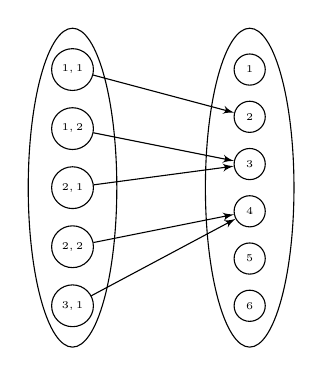
\begin{tikzpicture}[scale=.75, every node/.style={scale=.75}]
\tikzset{vertex/.style = {shape=circle,draw,minimum size=1.5em}}
\tikzset{edge/.style = {->,> = latex'}}

\draw (0, 2) ellipse (0.75cm and 2.7cm);

\node[vertex](a5) at (0,0) {\tiny $3,1$};
\node[vertex](a4) at (0,1) {\tiny $2,2$};
\node[vertex](a3) at (0,2) {\tiny $2,1$};
\node[vertex](a2) at (0,3) {\tiny $1,2$};
\node[vertex](a1) at (0,4) {\tiny $1,1$};

\draw (3, 2) ellipse (0.75cm and 2.7cm);

\node[vertex](b6) at (3,0)   {\tiny  $6$};
\node[vertex](b5) at (3,0.8) {\tiny  $5$};
\node[vertex](b4) at (3,1.6) {\tiny  $4$};
\node[vertex](b3) at (3,2.4) {\tiny  $3$};
\node[vertex](b2) at (3,3.2) {\tiny  $2$};
\node[vertex](b1) at (3,4) {\tiny    $1$};

\draw[edge] (a1) to (b2);
\draw[edge] (a2) to (b3);
\draw[edge] (a3) to (b3);
\draw[edge] (a4) to (b4);
\draw[edge] (a5) to (b4);

\end{tikzpicture}
}
\qquad
\subcaptionbox*{Partial Function}[.4\linewidth]{
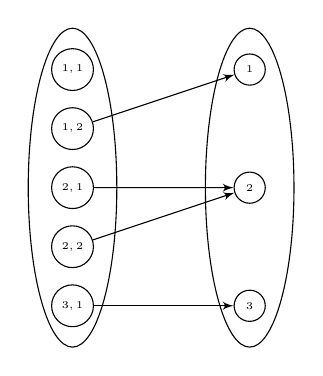
\begin{tikzpicture}[scale=.75, every node/.style={scale=.75}]
\tikzset{vertex/.style = {shape=circle,draw,minimum size=1.5em}}
\tikzset{edge/.style = {->,> = latex'}}
\draw (0, 2) ellipse (0.75cm and 2.7cm);

\node[vertex](a5) at (0,0) {\tiny $3,1$};
\node[vertex](a4) at (0,1) {\tiny $2,2$};
\node[vertex](a3) at (0,2) {\tiny $2,1$};
\node[vertex](a2) at (0,3) {\tiny $1,2$};
\node[vertex](a1) at (0,4) {\tiny $1,1$};

\draw (3, 2) ellipse (0.75cm and 2.7cm);

\node[vertex](b3) at (3,0)   {\tiny  $3$};
\node[vertex](b2) at (3,2) {\tiny  $2$};
\node[vertex](b1) at (3,4) {\tiny  $1$};

\draw[edge] (a2) to (b1);
\draw[edge] (a3) to (b2);
\draw[edge] (a4) to (b2);
\draw[edge] (a5) to (b3);

\end{tikzpicture}
}

\end{figure}

\end{slide}

\begin{slide}[bm=,toc=]{Injective / one-to-one Functions}
\begin{defn}{A.23}[Ben Ari]
$\mathcal{F}$ is \emph{injective} or \emph{one-to-one} if and only if
\[
  (x_1,...,x_{n-1}) \neq (y_1,...,y_{n-1})
\] 
\centering
implies
\[
  \mathcal{F}(x_1,...,x_{n-1}) \neq \mathcal{F}(y_1,...,y_{n-1})
\]

\end{defn}
\vspace{-5mm}
\begin{figure}[b]
\subcaptionbox*{Injective}[.4\linewidth]{
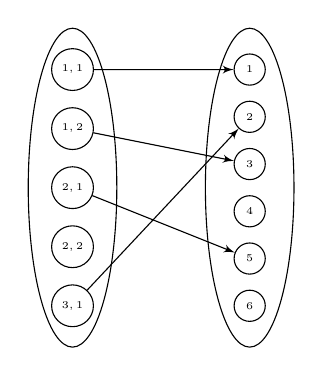
\begin{tikzpicture}[scale=.75, every node/.style={scale=.75}]
\tikzset{vertex/.style = {shape=circle,draw,minimum size=1.5em}}
\tikzset{edge/.style = {->,> = latex'}}

\draw (0, 2) ellipse (0.75cm and 2.7cm);

\node[vertex](a5) at (0,0) {\tiny $3,1$};
\node[vertex](a4) at (0,1) {\tiny $2,2$};
\node[vertex](a3) at (0,2) {\tiny $2,1$};
\node[vertex](a2) at (0,3) {\tiny $1,2$};
\node[vertex](a1) at (0,4) {\tiny $1,1$};

\draw (3, 2) ellipse (0.75cm and 2.7cm);

\node[vertex](b6) at (3,0)   {\tiny  $6$};
\node[vertex](b5) at (3,0.8) {\tiny  $5$};
\node[vertex](b4) at (3,1.6) {\tiny  $4$};
\node[vertex](b3) at (3,2.4) {\tiny  $3$};
\node[vertex](b2) at (3,3.2) {\tiny  $2$};
\node[vertex](b1) at (3,4) {\tiny    $1$};

\draw[edge] (a1) to (b1);
\draw[edge] (a2) to (b3);
\draw[edge] (a3) to (b5);
\draw[edge] (a5) to (b2);
\end{tikzpicture}
}
\qquad
\subcaptionbox*{Not Injective}[.4\linewidth]{
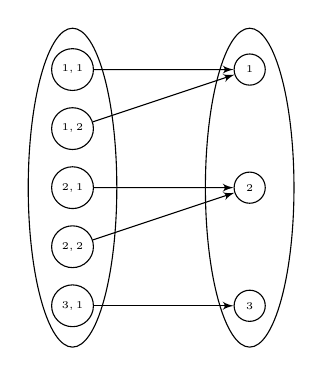
\begin{tikzpicture}[scale=.75, every node/.style={scale=.75}]
\tikzset{vertex/.style = {shape=circle,draw,minimum size=1.5em}}
\tikzset{edge/.style = {->,> = latex'}}
\draw (0, 2) ellipse (0.75cm and 2.7cm);

\node[vertex](a5) at (0,0) {\tiny $3,1$};
\node[vertex](a4) at (0,1) {\tiny $2,2$};
\node[vertex](a3) at (0,2) {\tiny $2,1$};
\node[vertex](a2) at (0,3) {\tiny $1,2$};
\node[vertex](a1) at (0,4) {\tiny $1,1$};

\draw (3, 2) ellipse (0.75cm and 2.7cm);

\node[vertex](b3) at (3,0)   {\tiny  $3$};
\node[vertex](b2) at (3,2) {\tiny  $2$};
\node[vertex](b1) at (3,4) {\tiny  $1$};

\draw[edge] (a1) to (b1);
\draw[edge] (a2) to (b1);
\draw[edge] (a3) to (b2);
\draw[edge] (a4) to (b2);
\draw[edge] (a5) to (b3);

\end{tikzpicture}
}

\end{figure}


\end{slide}

\begin{slide}[bm=,toc=]{Surjective / onto Functions}
\begin{defn}{A.23}[Ben Ari]~\\
\begin{itemize}
\item  $\mathcal{F}$ is \emph{surjective} or \emph{onto} if and only if
its range is all of $S_n$.
\item Equivalently,$\mathcal{F}$ from $S_1$ to $S_2$ is \emph{surjective} if 
and only if for all $y \in S_2$ there is a $x \in S_1$ such that
$\mathcal{F}(x) = y$. 
\end{itemize}
\end{defn}
\vspace{-5mm}
\begin{figure}[b]
\subcaptionbox*{Surjective}[.4\linewidth]{
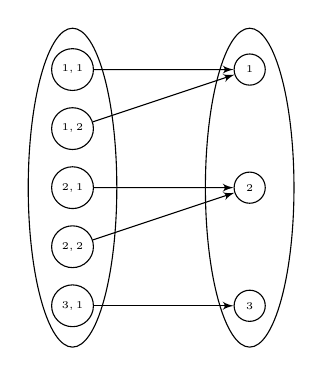
\begin{tikzpicture}[scale=.75, every node/.style={scale=.75}]
\tikzset{vertex/.style = {shape=circle,draw,minimum size=1.5em}}
\tikzset{edge/.style = {->,> = latex'}}
\draw (0, 2) ellipse (0.75cm and 2.7cm);

\node[vertex](a5) at (0,0) {\tiny $3,1$};
\node[vertex](a4) at (0,1) {\tiny $2,2$};
\node[vertex](a3) at (0,2) {\tiny $2,1$};
\node[vertex](a2) at (0,3) {\tiny $1,2$};
\node[vertex](a1) at (0,4) {\tiny $1,1$};

\draw (3, 2) ellipse (0.75cm and 2.7cm);

\node[vertex](b3) at (3,0)   {\tiny  $3$};
\node[vertex](b2) at (3,2) {\tiny  $2$};
\node[vertex](b1) at (3,4) {\tiny  $1$};

\draw[edge] (a1) to (b1);
\draw[edge] (a2) to (b1);
\draw[edge] (a3) to (b2);
\draw[edge] (a4) to (b2);
\draw[edge] (a5) to (b3);

\end{tikzpicture}
}
\qquad
\subcaptionbox*{Not Surjective}[.4\linewidth]{
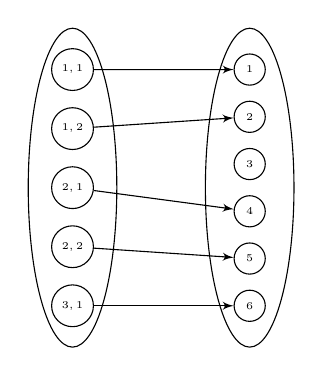
\begin{tikzpicture}[scale=.75, every node/.style={scale=.75}]
\tikzset{vertex/.style = {shape=circle,draw,minimum size=1.5em}}
\tikzset{edge/.style = {->,> = latex'}}

\draw (0, 2) ellipse (0.75cm and 2.7cm);

\node[vertex](a5) at (0,0) {\tiny $3,1$};
\node[vertex](a4) at (0,1) {\tiny $2,2$};
\node[vertex](a3) at (0,2) {\tiny $2,1$};
\node[vertex](a2) at (0,3) {\tiny $1,2$};
\node[vertex](a1) at (0,4) {\tiny $1,1$};

\draw (3, 2) ellipse (0.75cm and 2.7cm);

\node[vertex](b6) at (3,0)   {\tiny  $6$};
\node[vertex](b5) at (3,0.8) {\tiny  $5$};
\node[vertex](b4) at (3,1.6) {\tiny  $4$};
\node[vertex](b3) at (3,2.4) {\tiny  $3$};
\node[vertex](b2) at (3,3.2) {\tiny  $2$};
\node[vertex](b1) at (3,4) {\tiny    $1$};

\draw[edge] (a1) to (b1);
\draw[edge] (a2) to (b2);
\draw[edge] (a3) to (b4);
\draw[edge] (a4) to (b5);
\draw[edge] (a5) to (b6);

\end{tikzpicture}
}

\end{figure}

\end{slide}

\begin{slide}[bm=,toc=]{Bijective Functions}
\begin{defn}{A.23}[Ben Ari]~\\
$\mathcal{F}$ is \emph{bijective} or \emph{one-to-one and onto} if and only if
it is injective and surjective.
\end{defn}

\begin{figure}[b]
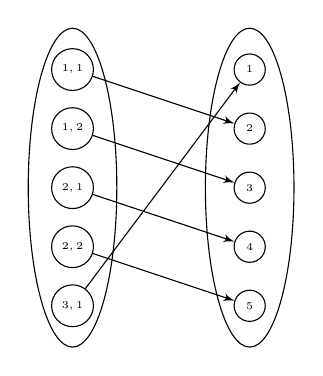
\begin{tikzpicture}[scale=.75, every node/.style={scale=.75}]
\tikzset{vertex/.style = {shape=circle,draw,minimum size=1.5em}}
\tikzset{edge/.style = {->,> = latex'}}

\draw (0, 2) ellipse (0.75cm and 2.7cm);

\node[vertex](a5) at (0,0) {\tiny $3,1$};
\node[vertex](a4) at (0,1) {\tiny $2,2$};
\node[vertex](a3) at (0,2) {\tiny $2,1$};
\node[vertex](a2) at (0,3) {\tiny $1,2$};
\node[vertex](a1) at (0,4) {\tiny $1,1$};

\draw (3, 2) ellipse (0.75cm and 2.7cm);

\node[vertex](b5) at (3,0) {\tiny  $5$};
\node[vertex](b4) at (3,1) {\tiny  $4$};
\node[vertex](b3) at (3,2) {\tiny  $3$};
\node[vertex](b2) at (3,3) {\tiny  $2$};
\node[vertex](b1) at (3,4) {\tiny  $1$};

\draw[edge] (a1) to (b2);
\draw[edge] (a2) to (b3);
\draw[edge] (a3) to (b4);
\draw[edge] (a4) to (b5);
\draw[edge] (a5) to (b1);

\end{tikzpicture}
\caption*{Bijective Function}
\end{figure}

\end{slide}

\begin{slide}[bm=,toc=]{Composition of Functions}
As with relations, we can combine functions using the \emph{composition} operation, 
denoted $f \circ g$.
\begin{itemize}
\item Assume $g$ is a function from $S_1$ to $S_2$ and $f$ is a function from 
$S_3$ to $S_4$ and let $S = S_2 \cap S_3$.
\item The composition forms a new function on $S_1 \times S_4$, such that:
\[
  f \circ g(x) = f(g(x))
\]
\vspace{-5mm}
\item Note: since functions are relations, the above follows immediately from
the definition of composition of functions.
\end{itemize}
\vspace{-5mm}
\begin{figure}[b]
\begin{subfigure}{.3\linewidth}
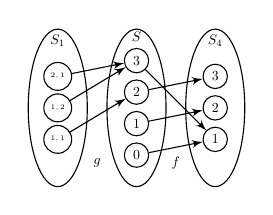
\begin{tikzpicture}[scale=.5, every node/.style={scale=.5}]
\tikzset{vertex/.style = {shape=circle,draw,minimum size=1.5em}}
\tikzset{edge/.style = {->,> = latex'}}

\draw (0, 1.2) ellipse (.75cm and 2cm);
\node[vertex](c) at (0,0.4) {\tiny $1,1$};
\node[vertex](b) at (0,1.2) {\tiny $1,2$};
\node[vertex](a) at (0,2)   {\tiny $2,1$};
\node (s1) at (0, 2.9) {$S_1$};

\node (g) at (1, -0.2) {$g$};

\draw (2, 1.2) ellipse (.75cm and 2cm);
\node[vertex](0) at (2,0) {$0$};
\node[vertex](1) at (2,0.8) {$1$};
\node[vertex](2) at (2,1.6) {$2$};
\node[vertex](3) at (2,2.4) {$3$};
\node (s) at (2, 3) {$S$};

\node (f) at (3, -0.2) {$f$};

\draw (4, 1.2) ellipse (.75cm and 2cm);
\node[vertex](b1) at (4,0.4) {$1$};
\node[vertex](b2) at (4,1.2) {$2$};
\node[vertex](b3) at (4,2)   {$3$};
\node (s4) at (4, 2.9) {$S_4$};

\draw[edge] (a) to (3);
\draw[edge] (b) to (3);
\draw[edge] (c) to (2);

\draw[edge] (0) to (b1);
\draw[edge] (1) to (b2);
\draw[edge] (2) to (b3);
\draw[edge] (3) to (b1);

\end{tikzpicture}

\end{subfigure}
\begin{subfigure}{.3\linewidth}
\begin{align*}
  f(x)       &= x \pmod{3} + 1 \\
  g(x_1,x_2) &= x_1 + x_2 \\
  f \circ g(x_1,x_2) &= f(g(x_1,x_2)) \\
                     &= (x_1 + x_2) \pmod{3} + 1
\end{align*}
\end{subfigure}
\end{figure}
\end{slide}

\end{document}

